% intro should describe and justify this cahpter
% 
\graphicspath{{chapters/3.Chapter_1/figures}}


\begin{savequote}[75mm]
"even after the observation of the frequent or constant conjunction of objects, we have no reason to draw any inference concerning any object beyond those of which we have had experience;"
\qauthor{- David Hume: \textit{A Treastie of Human Nature, 1738}}
\end{savequote}

\chapter{Endosymbiont Diversity}\label{chap:endo_diversity}

\section{Introduction}

\subsection{Endosymbiont taxonomy and clonality}

Over 50 strains of green algal photobionts have been identified in 
\textit{Paramecium bursaria} species \citep{Hoshina2010,Hoshina2004,Hoshina2009,Summerer2008,Vorobyev2009}. 
These form at least 4 distinct species groups:
\begin{itemize}
    \item \textit{Micractinium reisseri} 
    \item \textit{Chlorella variabilis}
    \item \textit{Chlorella vulgaris}
    \item \textit{Coccomyxa} sp. 
\end{itemize}
These form a paraphyletic distribution within the green algae
providing evidence for multiple separate origin events for
the \textit{P. bursaria} endosymbiosis \citep{Hoshina2008,Hoshina2009}
Furthermore, there is emerging evidence, in the form
of intron HGTs and sequencing that strains of \textit{P. bursaria}
are capabale of hosting double and triple co-habitations of different
photobiont species \citep{Hoshina2012}. Therefore,
before an effective analysis can take place of
an endosymbiotic system it is important
to carefully define the species involved. 

%variabilis = SAG211-6 (MRBG1), NC64A \citep{Blanc2010}
%reisseri = CCAP1660/12  and CCAP 221/83 (Pbi)
%vulgaris = CCAP1660/10
%coccomyxa = CCAP1660/13

Unfortunately, the systematics of the Chlorophyta has experienced a relatively
high degree of flux, with multiple redefinitions even since the initial 
use of molecular phylogenetics of ribosomal sequences \citep{Hori1985,Gunderson1987}
in the 1980s \citep{Leliaert2012,Hoshina2010}.  The algal endosymbionts of
\textit{Paramecium bursaria} in particular have gone through a range of 
names and classifications starting with \textit{Zoochlorella} in 1882 and
through various species of the genus \textit{Chlorella} \citep{Hoshina2010}.

Initially, all symbiotic algae were named as single \textit{Chlorella paramecii}
species but this name was rejected and \textit{Chlorella variabilis} 
was defined \citep{shihira1965chlorella} but this was in turn rejected and fell out of use.
Later, the first discovery of the existence of multiple distinct strains of photobiont was published \citep{Douglas1986}.
With this came the understanding that the endosymbionts of \textit{P. bursaria}
are likely to be divergent but not distinct species to other described
free-living \textit{Chlorella} \citep{Hoshina2010}.

To add further confusion to the system, the most recently
accepted terms defined species of endosymbiont merely 
as ``American'' and ``European''.  This lead to several
misidentifications (e.g. \citep{Kodama2007}) \citep{Hoshina2010}.
Recently, these two organisms have been redescribed as
distinct species \textit{Chlorella variabilis} and
\textit{Micractinium reisseri} respectively \citep{Hoshina2010}.
Therefore, care must be taken when reading older literature
to distinguish the earlier less well-defined \textit{C. variabilis}
from the modern usage.

One source of complication in the systematics of the photobionts have been
plagued with cases of mislabelling and loss of cultures
by various culture collections and in papers. For example, the initial culture
which the original \textit{Chlorella variabilis} was described from was lost
and a supposedly identical culture from a different collection
was found to have wildly different biochemical properties \citep{Hoshina2010}.
These complications and confusions add to the importance
of accurate endosymbiont species identification. 


The most widely accepted means of rapidly taxonomically profiling
archaeplastida (and indeed a range of eukaryote species) is that of 
nuclear ribosomal internal transcribed spacer 2 (ITS2) (see \cref{fig:its2_schematic}) barcoding. 
ITS2 has shown particular utility in the identification and separation
of closely related green algal species \citep{Buchheim2011} due to being
universal, reliably amplifiable and highly variable \citep{Hershkovitz1996}.

ITS2 barcoding has been recommended as a superior marker to 
other universal archaeplastida DNA barcodes such as the \textit{rbcL} 
\citep{Chen2010}.  The conserved nature of the flanking 5.8S and
18S sequences allows near universal primers to be designed which efficiently 
amplify ITS2 sequences unlike the broadly distributed but
highly variable \textit{rbcL} \citep{Buchheim2011}.

\begin{figure}[h]
    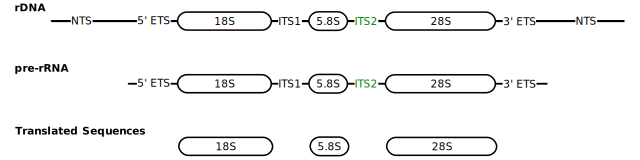
\includegraphics[width=\textwidth]{ITS_schematic.pdf}
    \caption{Structure of Eukaryotic nuclear ribosomal DNA.
        rRNA genes exist in tandem repeats separated by nontranscribed spacers (NTS).
        pre-rRNA contain 
    Redrawn from \citep{Shi2005}}
\label{fig;its2_schematic}
\end{figure}

Not only will ITS2 sequencing identify the endosymbiont species in
both CCAP 1660/12 and CCAP 1660/13 cultures, it will offer an
tool in which to investigate the presence of clonality within the
photobiont populations.  By sequencing a large number of 
ITS2 fragments amplified from the same culture there is a reasonably
good probability that all the ITS2 level diversity will be sampled. 
If on analysis of these sequences they form multiple clades or 
display divergent groupings this could be strong evidence
for a multiple photobiont co-habitation within the \textit{P. bursaria}
host. 


Finally, one last means in which we saught 
gain additional insight into the host-endosymbiont
system was through the use of multiple-displacement amplification (MDA)
based sequencing. Due to difficulties in obtaining sufficient
culture densities and the prevalence of putative sources of contamination
within the culture bulk genome sequencing was considered to be prone to 
major difficulties.  Therefore, MDA offered a way in which 
we could further investigate this question of photobiont clonality
while also generating a resources with potential use for further analysis.



%However, this type of barcoding approach to species identification is 
%imperfect 
%
%It has been discovered that the rDNA-ITS2 sequence is uniform
%within each of the described groups of endosymbiont species/strains 
%
%\citep{(Hoshina et al. 2004, 2005; Gaponova et al. 2007; Summerer et al. 2008; Hoshina & Imamura 2008a; Luo et al. 2010).
%with up to 20\% differences in the ITS2 (despite very similar exonic SSU rRNA)
%
%Species concepts  - ITS2 vs 18S vs whatever \citep{Boenigk2012}


%Assembly of mini-metagenomes/sc genomes \citep{Nurk2013}

\subsection{Isolation of hosts}

One avenue that is important for an effective analysis of a host-endosymbiont
system is the ability to analyse the partners in isolation.  This can be used
to test individual hypotheses regarding each partner and allowing controlled
reintroduction experiments. 
Unfortunately,
the majority of extant well-characterised endosymbioses display metabolic co-depdendence
and therefore, host and endosymbiont cannot be isolated without one or other dying. 

Fortunately, there have been numerous studies investigating this within the \textit{Paramecium bursaria}
- \textit{Chlorella/Micractinium} system.  %<> citations

Foremost among these is the only previously completed transcriptomic analysis of this system by \citep{Kodama2014c}.
 This analysis investigatedthe differential global metatranscriptome profile of \textit{P. bursaria} Yad1g strain with 
 and without its \textit{Chlorella variabilis} 1N endosymbiont 
\citep{Kodama2014c}.   While, this is a different strain of both host and endosymbiont to the CCAP1660/12 strains (\textit{P. bursaria} and \textit{Micractinium reisseri}) 
used in this thesis it offers a potential avenue to investigate these other components.  

Due to the presence of this existing analysis (and the data from it) we attempted to reproduce this
host isolation with the CCAP1660/12 strain. There have been several published methods
for clearing endosymbionts from host cells namely, the herbicide paraquat \citep{Hosoya1995a}, 
culturing under constant dark \citep{Karakashian1963}, herbicide DCMU \citep{Reisser1976},
X-ray \citep{Wichterman1948}, and cyclohexamide \citep{Weis1984,Kodama2007}.
As the most recent analyses tend to use paraquat, cyclohexamide, DCMU
and constant darkness \citep{Kodama2009a}.  These methods were used. 


Another avenue of study that we did not invstigate was that of
isolation of endosymbiont into free-living cultures. 
Unfortunately, the established fastidiousness of \textit{Micractinium reisseri} 
and \textit{Chlorella variabilis} species outwith their host, the relative
paucity of free-living examples of these species (to my knowledge
the only characterised strain is that described in \citep{Abou-Shanab2014}), 
and the relative variance in efficiency of the established methods
 \citep{Achilles-Day2013a}. This was not attempted. 



\section{Aim}

In this chapter I will determine the exact algal endosymbiont strains present
in the principal \textit{Paramecium bursaria} cultures used throughout
this thesis and their relationships relative to one another and to
other green algae. 

I will also use this data and single cell genomics to investigate whether the algal
endosymbiont present in the \textit{Paramecium bursaria-Micractinium reisseri}
CCAP 1660/12 strains form a clonal population. 

Finally, I will discuss the attempts to remove the endosymbiont in the 
\textit{Paramecium bursaria} CCAP 1660/12 strain from the host.

\section{Methods}

\subsection{Taxonomic Investigation}
    
\subsubsection{ITS2 Sequencing}

\textit{Paramecium bursaria} CCAP 1660/12 and \textit{Paramecium bursaria} CCAP 
1660/13 cultures were maintained in New Cereal Life (NCL) media
at \(18\celsius\) with 12:12 hour light/dark cycle.

ITS2 sequences were amplified from 3 separate biological replicates 



ITS2 sequences were amplified using ITS2-S2F and CHsp prime


\textit{Paramecium bursaria} 1660/13 ``Coccomyxa'' 
1k-10k used ITS2-S2F and ITS4-R
1D-3D using ITS2-S2F and CHsp
i


PCR products were then cleaned up, cloned, sequenced
and processed using the same protocol as \citep{Maguire2014a}.

Briefly, the successfully amplified PCR products were gel-purified 
(Wizard SV Gel and PCR Clean-Up kit, Promega).
These products were then TA-cloned 
using Agilent's PCR StrataClone Cloning Kit in a PSC-A-amp/kan
vector.
Successful clones were blue-white screened and 5 clones
selected for each PCR product.  
Clones were then externally Sanger sequenced using the M13Rev primer
at MWG Eurofins. 


Flanking vector and primer sequences were removed: sequenced trimmed to 
areas of high chromatograph quality and ambiguously defined bases corrected
using Sequencher \citep{Sequencher}.


From the 3 \textit{Paramecium bursaria} CCAP 1660/12 biological replicates
14, 9, and 11 ITS2 sequences were obtained respectively.





In order to mitigate the risk of sequencing error masquerading
as true sequence divergene any sequences found in later phylogenetic
analysis to demonstrate single nucleotide changes from the consensus
of its clade placement was resequenced at MWG Eurofins in reverse 
using M13Uni.  Specifically, these were ITS-B18,
ITS-2, ITS-19, ITS-B6, ITS-B3, ITS-A7, ITS-6, ITS-B15,
ITS-10, ITS-9, ITS-15, and ITS-1.
If the reverse sequencing didn't demonstrate the same polymorphism as
the original forward sequencing it was considered to be a likely 
sequencing error artefact and the divergent sequence was removed. 


%\subsubsection{18S Sequence determination}
%
%All assembled transcriptome contigs were BLASTP 
%against all Chlorella 18S sequenced from 
%\citep{Imamura2008}.

\subsubsection{Phylogenetics}

ITS2 sequences used in \citep{Hoshina2010}, \citep{Hoshina2013} were retrieved
from genbank. 

The trimmed sequences and the established database sequences were then
aligned using MUSCLE. This alignment was manually masked in the graphical seaview
tool.  The masked alignment was then run through jmodeltest to 
determine an appropriate substitution model. 
Finally, the alignment was used to generate both RaXML and 
MrBayes phylogenies . 







\subsection{Single Cell Genomics}

\subsubsection{DNA Extraction}

Individual \textit{P. bursaria} CCAP 1660/12 cells were removed from culture 
and washed three times in a successive series of 
\(10 \mu l\) drops of sterile modified 
New Cereal Leaf-Prescott (NCL) medium to minimise prokaryotic contamination from 
bacterial foodstocks in the culture media. 
Cells were added to a final \(10\mu l\) drop of sterile water before being added
to a microcentrifuge tube.

DNA was then extracted using a Cetrimonium bromide based method adapted from \citep{Winnepenninckx1993}. 
In brief,  \(748.5 \mu l\) of CTAB extraction buffer (at \(37\celsius\) and \(100 \mu l\) beads (Sigma, \(425 – 600 \mu m\); acid washed) 
were added and the tube was vortexed for 5 minutes. 
The tube was incubated for 50 minutes at \(37\celsius\), 
vortexed again for 5 minutes and incubated for 50 minutes at \(60\celsius\). 
DNA was extracted three times with phenol/chloroform/isoamylacohol (25:24:1, pH 8), washed with 70\% ethanol and 
re-suspended in \(2.5 \mu l\) TE (pH 8). 
Whole-genome amplification of purified genomic DNA was performed using the multiple-displacement amplification based
(MDA) Qiagen REPLI-g Single Cell Kit. 
The REPLI-g amplified gDNA was purified using a QIAamp DNA mini kit and eluted in \(100 \mu l\) elution buffer.

\subsubsection{Library Preparation}


\subsubsection{Illumina Sequencing}

5 prepared libraries were put forward for sequencing 
(Pb-3, Pb-4, Pb-6, Pb-7 and Pb-8).   Samples were
multiplexed and were rapid sequenced in an Illumina
HiSeq 2500 in 150bp paired-end mode. 

\subsubsection{Read pre-processing}

Trimmomatic \citep{Bolger2014a} was used to trim sequencing adapters (using sequences
provided by Exeter Sequencing Service) via the ILLUMINACLIP setting.
Reads were then quality trimmed at a minimum average SLIDINGWINDOW 
quality thresholds of Q5 and Q30. 

Q5 and Q30 trimmed reads were then error corrected using BayesHammer
\citep{Nikolenko2013} as built into the SPAdes assembler \citep{Bankevich2012}.

Trimmed and error corrected libraries were also then digitally normalised
\citep{Brown2012} to a coverage of 20 and with a K-mer size of 25.
K-mers were then abundancy filtered \citep{Zhang2014,Zhang2015}
using the Khmer package \citep{Crusoe2015}.

\subsubsection{Assembly}

Assemblies were then generated using the following sets
of data:
\begin{itemize}
    \item Q5 trimmed reads with error correction
    \item Q5 trimmed reads with error correction and digital normalisation/filtering
    \item Q30 trimmed reads with error correction
    \item Q30 trimmed reads with error correction and digital normalisation/filtering
\end{itemize}

The following assemblers were used:
\begin{itemize}
    \item SPAdes assembler \citep{Bankevich2012,Nurk2013}
    \item SPades assembler with autocoverage thresholding 
    \item MEGAHIT \citep{Li2015a}
    \item Platanus \citep{Kajitani2014}
    \item SOAPdenovo2 \citep{Luo2012}
    \item Hybrid \textit{De novo} Assembler (HyDA) \citep{Movahedi2014}
\end{itemize}

\subsubsection{Assembly assessment}

Assemblies were assessed and compared using the
QUality ASsessment Tool for genome assembly (QUAST) \citep{Gurevich2013a}
and key assembly metrics were compared (N50, N90, contig number
and length and total assembly size).


%hagfish?


\subsubsection{Assembly decomposition}

Contigs were subsequently cut into 10kb fragments for consistency
in binning and taxonomic assignment.
Reads were mapped back onto the final assembly using Bowtie2 
\citep{Langmead2012} 

Using the metagenomic binning tool, CONCOCT \citep{Alneberg2014}
contigs were binned into clusters based on sequence composition
and coverage features (derived from mapping data).
Coverage features were derived from a coverage and linkage table
generated via CONCOCT scripts built around BEDTools \citep{Quinlan2010,Quinlan2014}, Picard \url{http://broadinstitute.github.io/picard/} 
and Samtools \citep{Li2009} 
based parsing
of the bowtie2 alignment files.
Clustering was conducted using a Gaussian Mixture Model (GMM) \citep{Bishop2006}
and the number of clusters determined through variational Bayesian inference \citep{Corduneanu2001}.

All CONCOCT analyses were completed using a provided pre-configured 
Docker Image \citep{Merkel2014}, a form of lightweight 
distributable process isolation container.
This was downloaded from DockerHub \url{https://hub.docker.com/r/binpro/concoct/}
on 2015-10-25.

Additionally, the cut contigs were taxonomically assigned 
using TAXAssign \url{https://github.com/umerijaz/TAXAassign} against the NCBI nt database. 
The BLAST database was downloaded using update\_blastdb.pl script \url{http://www.ncbi.nlm.nih.gov/blast/docs/update_blastdb.pl}
and TAXAssign was run in parallel (using GNU parallel \citep{Tange2011a})
with a maximum of 10 reference matches
per contig a minimum percentage identity for assignment
to a given taxonomic level of 60, 70, 80, 95, 95, and 97
for Phylum, Class, Order, Family, Genus and Species respectively. 

CONCOCT clusters were then evaluated using the taxonomic assignments from TAXAssign
using the provided ``validate.pl'' script.

\subsubsection{Assembly annotation}
Orphelia \citep{Hoff2009}
MetaGUN \citep{Liu2013}

Final, candidate assemblies were then analysed using 
Bencmarking Universal Single-Copy Orthologs (BUSCO) \citep{Simao2015}

\subsection{Endosymbiont elimination}

CCAP 1660/12 and YADGN1 cultures in NCL media with were treated under the following
conditions to attempt to remove the endosymbiont. 
\textit{P. tetaurelia} were used as a control culture and was
given the same treatment. 

Paraquat was added at both \(1mg\mu l^{-1}\) and
\(0.5mg\mu l^{-1}\) concentrations.
Cultures were maintained under normal 12:12 lit:dark 
conditions at \(15\celsius\).  Cultures were inspected
daily using light microscopy and assessed for ``bleaching''.

Cyclohexamide was added to cultures at both \(1mg\mu l^{-1}\)
and \(10mg\mu l^{-1}\), again cultures were maintained under
standard 12:12 lit:dark condition and \(15\celsius\). 
Cultures when looking clear were subcultured and resuspended in 
NCL without cyclohexamide.

Cultures were maintained in the dark without a lit phase
at \(15\celsius\) and inspected every 2 weeks for clearing.
This was to prevent providing too much light and 
further encouraging endosymbiont growth. 

\section{Results}

\subsection{ITS2 Phylogeny}


As CHSP primer wasn't homologous to \textit{Coccomyxa} 
at the 3' prime end we used ITS4R

but if it wasn't homologous why was it the same?


\subsection{18S Fragment Phylogeny}

All assembled contigs from final transcriptome assembly (see \ref{chap:})


\subsection{Single Cell Genomes}

\subsubsection{Sequencing and Pre-processing}

\begin{table}
    \begin{tabular}{|c|c|c|}
        \hline
        \textbf{Sample} & \textbf{Raw PE Reads} & \textbf{Q30 Trimmed PE Reads} & \textbf{Q5 Trimmed PE Reads}\\
        \hline
        Pb-3 & \(3.523\cdot10^7\) & \(1.951\cdot10^7\) & \(2.737\cdot10^7\) \\
        Pb-4 & \(3.228\cdot10^7\) & \(2.606\cdot10^7\) & \(3.035\cdot10^7\) \\
        Pb-6 & \(3.291\cdot10^7\) & \(2.437\cdot10^7\) & \(2.962\cdot10^7\) \\
        Pb-7 & \(4.023\cdot10^7\) & \(2.642\cdot10^7\) & \(3.404\cdot10^7\) \\
        Pb-8 & \(3.869\cdot10^7\) & \(2.613\cdot10^7\) & \(3.246\cdot10^7\) \\
        \hline
    \end{tabular}
\end{table}





\subsubsection{Assembly}


Spades Q5 assembly

\begin{table}
\begin{tabular}{|l*{4}{|r}|}
\hline
Assembly & scaffolds broken & scaffolds & contigs broken & contigs \\ \hline
\# contigs ($\geq$ 0 bp) & 93950 & {\bf 92720} & 94384 & 94384 \\ \hline
\# contigs ($\geq$ 1000 bp) & 12293 & {\bf 11913} & 12614 & 12614 \\ \hline
Total length ($\geq$ 0 bp) & 81560052 & {\bf 81653830} & 81478234 & 81478234 \\ \hline
Total length ($\geq$ 1000 bp) & 58290298 & {\bf 58754139} & 58162565 & 58162565 \\ \hline
\# contigs & 23762 & {\bf 23105} & 24109 & 24109 \\ \hline
Largest contig & 209873 & 209873 & 209873 & 209873 \\ \hline
Total length & 66173340 & {\bf 66443935} & 66064486 & 66064486 \\ \hline
GC (\%) & 39.26 & 39.27 & 39.27 & 39.27 \\ \hline
N50 & 6638 & {\bf 7117} & 6334 & 6334 \\ \hline
N75 & 2232 & {\bf 2411} & 2188 & 2188 \\ \hline
L50 & 2090 & {\bf 1983} & 2241 & 2241 \\ \hline
L75 & 6426 & {\bf 6047} & 6716 & 6716 \\ \hline
\# N's per 100 kbp & 0.93 & 141.64 & {\bf 0.00} & {\bf 0.00} \\ \hline
\end{tabular}
\caption{Spades Q5 assembly 
All statistics are based on contigs of size $\geq$ 501 bp, unless otherwise noted (e.g., "\# contigs ($\geq$ 0 bp)" and "Total length ($\geq$ 0 bp)" include all contigs).}
\end{table}






\subsubsection{Binning}

\begin{figure}
	\includegraphics[width=\textwidth]{CONCOCT_clusters.pdf}
	\caption{A low dimensional Principal Component representation of genomic contig
		cluster assignments.  Clusters are assigned via a Gaussian Mixture Model (GMM) 
		based on sequence compositional and coverage features as implemented in CONCOCT.
		Unfortunately, as can be observed clusters are both poorly distinguished even
		in the dimensions of the 2 principal components (PCA1 and PCA2) and are numerous (34). 
	\label{fig:concoct_clusters}
\end{figure}


TAXAssign assigned 3,037 labels to the 11,757 contigs. 
\begin{table}
	\begin{tabular}{r | l c |}
\textbf{Source Group} & \textbf{Number of Contigs} & \textbf{Phylum-Level Breakdown} \\
\hline
\textbf{Host} & 13 & Intramacronucleata\\
- & 2  & Apicomplexa\\
- & 1  & Colponemidia \\
\hline 
\textbf{Endosymbiont} & 12 & Chlorophyta\\
- &  12 & Streptophyta\\
- &  1 & Cyanobacteria\\
\hline
\textbf{Bacterial Contamination} & 16230 & Proteobacteria \\
- & 468 & Firmicutes\\
- & 329 & Actinobacteria\\
- & 128 & Bacteroidetes/Chlorobi group\\
- & 1 & Deinococcus-Thermus\\
\hline
\textbf{Eukaryotic Contamination} & 605 & Ascomycota \\
 - & 380 & Chordata\\
 - & 74 & Arthropoda \\
 - & 12 & Basidiomycota\\
- & 7  & Nematoda \\
- & 1 & Platyhelminthes\\
- & 1 & Cnidaria\\
\hline
\textbf{Unknown} & 540 & Unclassified \\
\hline
	\end{tabular}
	\caption{Summary of taxonomic assignments via TAXAassign grouped into putative ``source groups'' reflecting
		the most probable source of 10kb chunked contigs of that specific taxonomic provenance.  Of note, is the disproportionate
		number of contigs from contaminating sources. Specifically, }
	\label{}
\end{table}


    

Clusters were additionally validated by comparison to taxonomically BLASTN
assigned contig labels.    

11,757 contigs with 3,3037 were clustered into 34 unique clusters.
When these clusters were compared with a ``ground-truth'' from
the taxonomic assignment of clusters 

\begin{table}
	\begin{tabular}{| c || c | c |}
		 - & Positive & Negative \\
		 \hline
		 \hline
		True  &  Contigs with same taxonomic assignment are assigned to the same cluster  & Contigs with different taxonomic assignments are assigned to different clusters\\
		False &  Contigs with different taxonomic assignments are assigned to the same cluster  & Contigs with the same taxonomic assignment are assigned to different clusters \\
	\end{tabular}
	\caption{A contextual explanation of True and False Positive and Negatives in the context of contig binning/clustering.  Top left indicates what a
		True Positive (TP) means in this context, bottom left a False Positive (FP).  Similarly Top Right explains a True Negative (TN) and Bottom Right a
		False Negative (FN)}
	\label{tab:cluster_outcome_explanation}
\end{table}


Recall that Precision and Recall can be defined as follows:
\[Precision = \frac{TP){TP+FP}
Recall=\frac{TP}{TP+FN}\] 
where \(TP\) are True Positives and \(FP\) and \(FN\) are False Positives
and Negatives respectively (see \cref{tab:cluster_outcome_explanation} for an 
explanation of what these terms mean in the context of clustering).

CONCOCT assigned clusters were relatively precise \(0.912608\) 
therefore there were relatively few \(FP\) i.e. the majority of clusters 
contained contigs with the same taxonomic assignments. 

However, recall was relatively poor \(0.542250\) suggesting a
fair number of FN i.e. contigs with the same taxonomic assignments
were not confined to a single cluster and were spread over main clusters.

The \(F_1\)\footnote{\(F_1 = 2 * \frac{precision * recall)}{[precision + recall]}\)} score for CONCOCT 
clustering was therefore \(0.680389\) under the, slightly flawed, assumption that 
TAXAssign represents the ground-truth.

It is also worth noting that the 34 clusters had a relatively high level of mutual information
(Normalised Mutual Information of \(0.332022\) and a Rand Index of \(0.499741\)) suggesting
many small but highly similar clusters were created.  This level of similarity combined
with the poor recall suggests a greater number of clusters were necessarily present in the
ground-truth.

\subsection{Elimination}

After 1 week \(10\mu g ml^{-1}\) Paraquat cultures were partially bleached. 
Unfortunately, after 2 weeks and despite regular feeding all \textit{Paramecium}
were also dead. The same pattern was observed with \(1\mu g ml^{-1}\) treated
cultures just a slower process.   After 6 weeks, cultures began to clear
and then promptly died. 

A similar pattern was observed with both concentrations of
cycloheximide where \(10\mu g ml^{-1}\) treatment 
led to a reduction in endosymbiont abundance by 90\%
after 1 week followed promptly by host death. 
The lower concentration \(1\mu g ml^{-1}\) 
displayed the same pattern but over a 6 week period.

Finally, with subculturing and feeding cultures maintained in 
constant darkness did lead to gradual bleaching over 4-8 weeks.
However, after 10 weeks the cultures ended up dead. 


\section{Discussion}

Group I introns may have been transmitted between \textit{C. variabilis}
and \textit{M. reisseri} strains during sympatric co-habitation
of the a common host \citep{Hoshina2012}. 
Endosymbiont switching could potentially occur by two scenarios
loss and replacement or co-symbiosis and replacement \citep{Hoshina2012}.
%This diversity of endosymbiotic origins in \textit{P. bursaria}
%coupled with multiple endosymbioses in a range of other
%eukaryotic species (e.g. Amoebozoa, Rhizaria, and Stramenopiles)
%suggests that these green algae may have several pre-adaptations
%that particularly suit them to forming endosymbiosies with a diverge range
%of hosts \citep{Gomaa2014}.
As the photobiont is vertically inherited in the host
\citep{Siegel1960}. 



\subsection{Reliability of Culture Collection}

The clear result is that despite the \textit{Paramecium bursaria} CCAP 1660/13
supposedly containing a \textit{Coccomyxa} endosymbiont 
all ITS2 sequences from this culture differeed fromt he published
\textit{Coccomyxa} sequence (accession \(AB260896.1\)) and were identical
to those sequences from the \textit{Paramecium bursaria} CCAP 1660/12 \textit{Micractinium
reisseri} endosymbiont.



Unfortunately, on communication with CCAP it emerged that they lost
the CCAP 1660/11 and 1660/12 strains in their collection. 


CCAP 1660/13 had become overgrown by free-living \textit{Coccomyxa}. 

However, it emerged that despite previous findings that CCAP 1660/13
did appear to contain the \textit{Coccomyxa} by \citep{Imamura2008} this was
likely to be contamination from the \textit{Coccomyxa} in the media as 
the CCAP 1660/12 and CCAP 1660/13 cultures were isolated from the same
pond (Cambridge, UK) by CCAP and appear to both have \textit{Micractinium
reisseri} endosymbionts.

This was confirmed by our ITS2 analysis.


However, this all demonstrates clear evidence of not taking previous studies
or culture collection descriptions without careful consideration.





taxonomic resolution - barcoding?
ITS2 sequencing could be improvied - possible sequencing error 



This also demonstrates the importance of isolating the algae
before sequencing to ensure population analysis isn't
contaminated with culture based representatives \citep{Achilles-Day2013a}.



The majority of ITS2 based studies make use of the secondary structure (predicted
using tools such as RNAstructure \citep{Mathews2004}) in inference \citep{Schultz2009}. 
This increases reliability of phylogenetic inference \citep{Keller2008} allows ITS2 to be used
to distinguish higher taxonomic levels \citep{Coleman2003}, and plays a role
in resolving the thorny problem of species determination \citep{Muller2007}. 
However, as the endosymbiont species ITS2 secondary structures have already been extensively
investigated (e.g. \citep{Hoshina2008,Hoshina2010}) it was considered an unneccessary 
analysis that would be unlikely to change the placment of any taxa in
this sequencing analysis. 



%With the exception of \textit{Chlorella variabilis} \citep{Blanc2010}
%representatives of all 3 other endosymbiont species groups 
%have been found to contain free-living strains.  In fact,
%the majority of described strains of \textit{Coccomyxa} \citep{Blanc2012}
%and \textit{C. vulgaris} are free-living.  On the other hand,
%only one free-living strain of \textit{M. reisseri} \citep{Abou-Shanab2014} 
%has been described.  The paucity of free-living strains
%within \textit{C. variabilis} and \textit{M. reisseri} is hypothesised by \citep{Hoshina2012}
%to be related to their nutritional fastidiousness \citep{Achilles-Day2013a,Kamako2005}
%and predation by a pair of \textit{P. bursaria}-\textit{Chlorella} viruses (PBCV)\footnote{
%    Strictly, that should be a PBCV and one \textit{P. bursaria} - \textit{Micractinium} virus,
%however, all literature relating to these viruses refers to PBCV.}
%\citep{Reisser1988}. 




\subsection{Clonality of endosymbionts}

The biases induced by MDA in single cell genomes are known to be 
formation of chimeric sequences and the amplification
of undesired contaminant sequences \citep{Binga2008}.

Additionally, despite a theoretical basis that
the amplification coverage bias should be random \citep{Hosono2003}
there is evidence disputing this in practice \citep{Ellegaard2013}.
The magnitude of this bias is related to the starting
quantity of DNA \citep{Ellegaard2013a}.

Fortunately, there does not appear to be any bias
related to GC \citep{Ellegaard2013a}


An increase in the number of starting cells to the range of
a few hundred to a few thousand bacterial cells
improves amplifciation considerably \citep{Ellegaard2013a}



The majority of tools focussing on the analysis
and assembly of single cell genomes are fixated
on bacterial systems near exclusively. Take for example,
automation tools such as SmashCell 
The majority of tools focussing on the analysis
and assembly of single cell genomes are fixated
on bacterial systems near exclusively. Take for example,
automation tools such as Son{Diversity of traits in endosymbionts}

Due to the repeated failure to create endosymbiont free \textit{Paramecium}
hosts from the CCAP 1660/12 cultures using 3 of the major accepted
methodologies (cultivation in darkness \citep{Karakashian1963},
paraquat \citep{Hosoya1995a,Tanaka2002} or cycloheximide \citep{Weis1984effect})




Cycloheximide does partially inhibit host protein synthesis
\citep{Weis1984effect,Kodama2007,Kodama2008,Kodama2009a}
therefore it is possible that in the host strain found in the
CCAP 1660/12 culture that this partial inhibition is lethal to both
host and endosymbiont. 
Therefore, this is a weaker of evidence indicating that this
endosymbiosis is not facultative. 






One method that wasn't attempted was the use of 3-(3,4-dichlorophenyl)-1,1-dimethlyura (DCMU)
an established blocker of photosystem II \citep{Reisser1976}. 
However, DCMU has previously been found to be mildly toxic in \textit{P. bursaria}, 
affecting the sexual reproduction system \citep{Miwa2009} therefore, this would
have proven unlikely to resolve the issues.






While it is possible that 

Unless
Unless, the
\textit{P. bursaria} - \textit{C. variabilis} system studied by \citep{Kodama2014c}







This indicates the presence of key differences between the current state of this
endosymbiosis and the previously studied \textit{C. variabilis} endosymbiosis
studied by \citep{Kodama2014c}.


An attempt was made to replicate this work using the CCAP1660/12 strains, unfortunately, elimination of the endosymbionts without death of the host
didn't prove possible in these strains.  Despite using 
(despite earlier publications to the contrary) by either maintaining the culture in the dark \citep{Siegel1960} (although some studies have thrown doubt on
        how effective this method is at completely elimiating the photobiont \citep{Tanaka2002}) or treatment with various titrations of herbicides 
            (e.g. paraquat \citep{Hosoya1995a}) or the protein synthesis inhibitor cyclohexamide \citep{weis1984effect}).\footnote{
        There are naturally aposymbiotic strains of \textit{Paramecium bursaria} \citep{Tonooka2002a}}




\section{Conclusions}

Therefore, on the basis of ITS2 sequencing the CCAP 1660/12 culture endosymbiont is
a strain of \textit{Micractinium reisseri}.  Additionally, the CCAP 1660/13
endosymbiont has been misclassified as a strain \textit{Coccomyxa} and
is the same \textit{Micractinium reisseri} species found in the CCAP 1660/12 
culture. Despite poor performance in genome assembly, the evidence of
the genomes and ITS2 data seem to indicate that this endosymbiont
forms a clonal or near clonal population within the CCAP 1660/12
endosymbiont.  At a minimum, a single strain of \textit{M. reisseri} 
comprises the sole green algal endosymbiont in the CCAP 1660/12
and 1660/13 cultures. 

Finally, this endosymbiont 



%Is it the species we think it is?
%Yes 18S/ITS2 among green algae

The \textit{Micractinium reissieri} endosymbiont in cultures CCAP 1660/12 
CCAP 1660/13 has potentially become metabolic co-dependent with the host.
The host appears incapable of survival without the endosymbiont.  
